\documentclass[tikz,border=10pt]{standalone}
\begin{document}
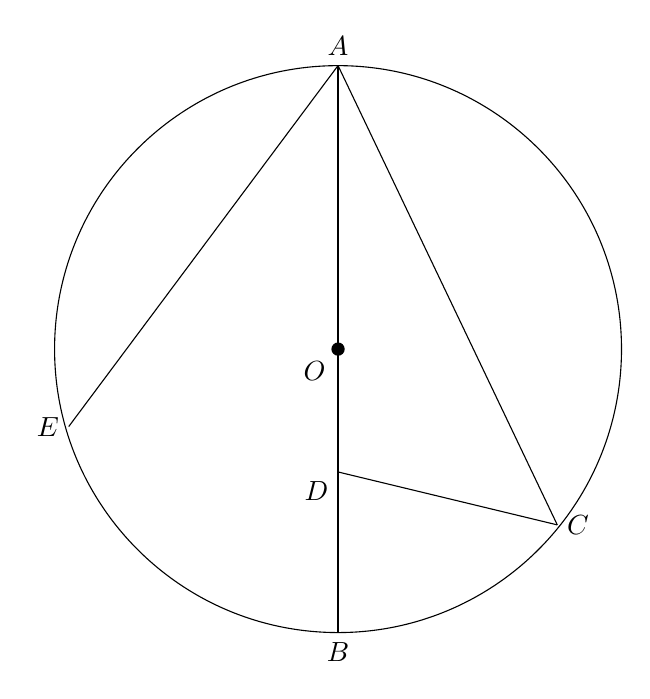
\begin{tikzpicture}[scale=1.2]
  \coordinate (O) at (0,0);
  \coordinate (A) at (0,3);
  \coordinate (B) at (0,-3);
  \coordinate (D) at (0,-1.3);
  \coordinate (E) at (-2.85,-0.82);
  \coordinate (C) at (2.32,-1.86);

  \draw (O) circle (3);
  \draw (A) -- (B);
  \draw (A) -- (E);
  \draw (A) -- (C);
  \draw (D) -- (C);

  \fill (O) circle (2pt);

  \node[above] at (A) {$A$};
  \node[below] at (B) {$B$};
  \node[below left=1pt] at (O) {$O$};
  \node[below left=0pt] at (D) {$D$};
  \node[left] at (E) {$E$};
  \node[right] at (C) {$C$};
\end{tikzpicture}
\end{document}
